%!TEX root = ../../deco_star.tex




\begin{table}
\tiny

% \begin{tabu} to \linewidth { |[.05mm middleGray] l |[.05mm middleGray] l |[.05mm middleGray]
%     % l
%     % g
%     % g
%     % g
%     % l
%     % l
%     % l
%     % l
%     % g
%     % g
%     % g
%     % l
%     % l
%     % l
%     X[1,l]
%     >{\columncolor[gray]{0.9}}X[1,c]
%     >{\columncolor[gray]{0.9}}X[1,c]
%     >{\columncolor[gray]{0.9}}X[1,c]
%     X[1,l]
%     X[1,l]
%     X[1,l]
%     X[1,l]
%     >{\columncolor[gray]{0.9}}X[1,c]
%     >{\columncolor[gray]{0.9}}X[1,c]
%     >{\columncolor[gray]{0.9}}X[1,c]
%     X[1,l]
%     X[1,l]
%     X[1,l]
%     |[.05mm middleGray]}
%     \taburulecolor{middleGray}\hline
%     % \tableHeaderStyle
%     \multicolumn{3}{|[.05mm middleGray]g}{} & 
%     \multicolumn{3}{g}{HOW} & 
%     \multicolumn{4}{g}{WHAT} &
%     \multicolumn{3}{g}{WHERE} & 
%     \multicolumn{3}{g|[.05mm middleGray]}{WHEN}
%     \\

%     \taburulecolor{middleGray}\hline

%     \multicolumn{2}{|[.05mm middleGray]l|[.05mm middleGray]}{} & 
%     \sidy{Total (out of 50)} & 
%     \sidy{File} & \sidy{UI} & \sidy{Canvas} & 
%     \sidy{Code} &  \sidy{Value} & \sidy{Intermediate} & \sidy{Element} &
%     \sidy{Global} & \sidy{Region} & \sidy{Local} &
%     \sidy{Before} & \sidy{During} & \sidy{After} 
%     \\

    
%     \taburulecolor{middleGray}\hline
%     \everyrow{\tabucline[.05mm  mainColor]{2-}}

%     & \multicolumn{15}{l|[.05mm middleGray]}{\textit{Setup}} \\
%     & \color{nicegray}{Configuration} & 13 & 13 & & & 9 & 4 & & & 13 & 2 & & 13 & &   \\
%     & \color{nicegray}{Initalization} & 20 & 18 & 3 & & 3 & 16 & 8 & 2 & 19 & 3 & & 20 & &   \\


%     \taburulecolor{middleGray}\hline
    
%     & \multicolumn{15}{l|[.05mm middleGray]}{\textit{Exemplars}} \\ 

%     \multirow[t]{19}{*}{\sidy{\hspace{-10em}$\longleftarrow$ \textit{Decreasing Automation}}}
%     & \color{nicegray}{Image} & 13 & 11 & 1 & & & & 12 & 2 & 13 & 2 & & 13 & &   \\
%     & \color{nicegray}{Arrangement} & 13 & 11 & 1 & 3 & 4 & & 3 & 10 & 13 & 4 & & 13 & 1 &  \\
%     & \color{nicegray}{Element} & 11 & 7 & 3 & 1 & & & 5 & 6 & 9 & 3 & & 11 & 1 &   \\


%     & \multicolumn{15}{l|[.05mm middleGray]}{\textit{Parameterization}} \\
%     & \color{nicegray}{Visual} Output  & 36 & 26 & 8 & & 5 & 30 & 2 & & 34 & 2 & & 19 & 1 & 19 \\
%     & \color{nicegray}{System} & 22 & 14 & 8 & & & 21 & 1 & & 23 & 4 & & 22 & 1 & \\

%     & \multicolumn{15}{l|[.05mm middleGray]}{\textit{Handling}} \\
%     & \color{nicegray}{Visual} UI & 10 & & 4 & 4 & & 1 & 7 & 4 & 7 & 6 & & 5 & 3 & 5 \\
%     & \color{nicegray}{Image} & 11 & 11 & & & 2 & & 9 & & 11 & 5 & & 11 & &   \\
%     & \color{nicegray}{Sketch} & 10 & & 1 & 9 & & & 10 & 5 & 6 & 9 & 2 & 8 & 3 & 2 \\


%     & \multicolumn{15}{l|[.05mm middleGray]}{\textit{Filling}} \\
%     & \color{nicegray}{Shapes} & 41 & 32 & & 11 & 26 & & 14 & & 40 & 15 & & 41 & 3 &   \\
%     & \color{nicegray}{Masking} & 11 & 5 & & 8 & 2 & & 9 & & 8 & 11 & & 11 & 2 &   \\
%     & \color{nicegray}{Curve} & 9 & & & 9 & & & 7 & 2 & 1 & 9 & & 8 & 2 &   \\


%     & \multicolumn{15}{l|[.05mm middleGray]}{\textit{Guiding}} \\
%     & \color{nicegray}{Brushing} & 8 & 1 & & 7 & & & 2 & 6 & 2 & 8 & & 2 & 7 &    \\
%     & \color{nicegray}{Directions} & 9 & 1 & & 8 & & & 8 & 1 & 8 & 8 & & 9 & &   \\



%     & \multicolumn{15}{l|[.05mm middleGray]}{\textit{Placing}} \\
%     & \color{nicegray}{Element} & 9 & & & 9 & & & & 9 & & 1 & 9 & 9 & 2 & 1  \\
%     & \color{nicegray}{Drag\&Drop} & 7 & & & 7 & & & & 7 & 1 & 5 & 6 & & 6 & 3 \\

%      \taburulecolor{middleGray}\hline


% \end{tabu}


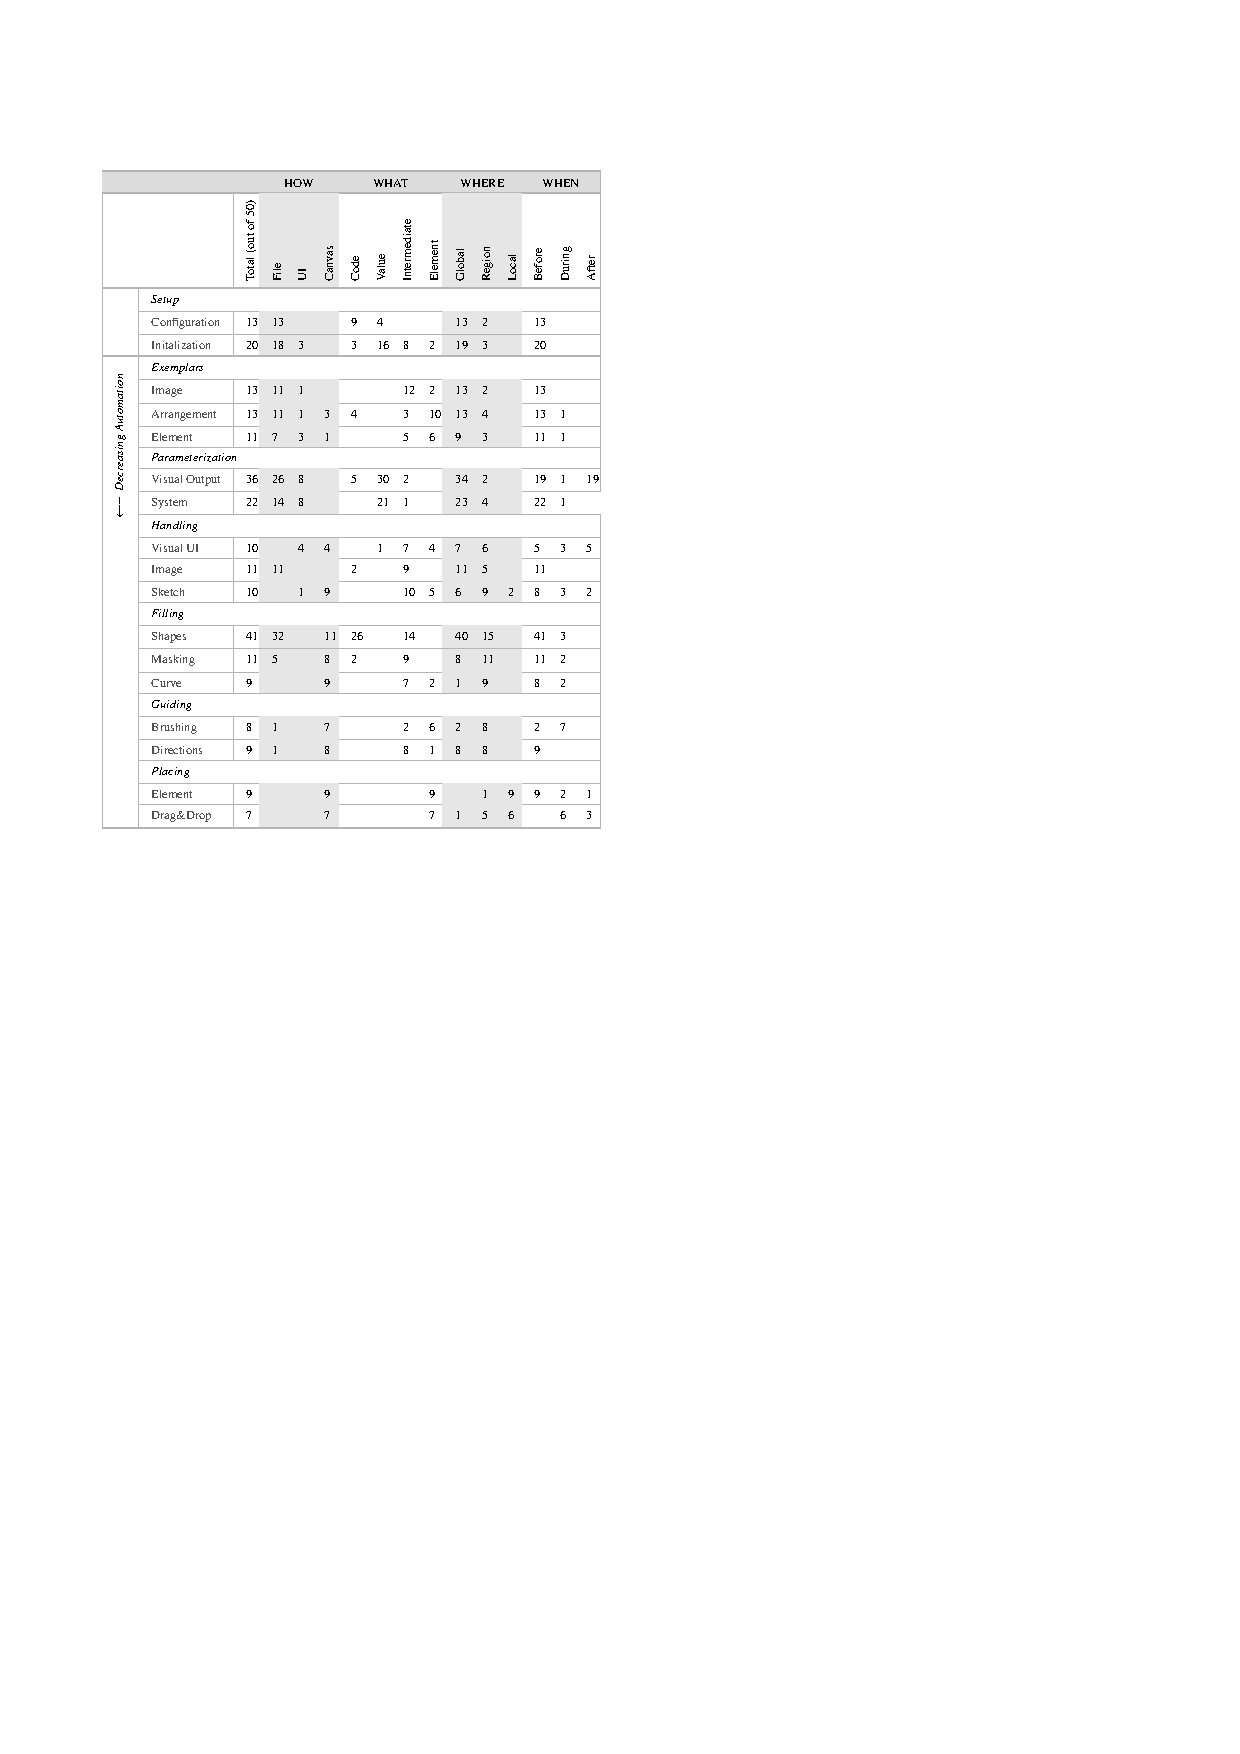
\includegraphics[width=\linewidth]{tables/table_controlmechanism.pdf}

\caption[Prevalence of control mechanisms]{Prevalence of control mechanisms in the literature: In total, 50 publications are included (the discussed state of the art work). Please note, that the totals of each step (how, what, where, when) can exceed the total of that category as it can be implemented within multiple usage scenarios.\label{table:taxo_controlmechanism}}
\end{table}
